% chapters/dataset.tex

% Section 3: Dataset, Preprocessing and Data Augmentation

% Frame 1: Dataset Origin
\begin{frame}{Dataset}
  \begin{itemize}
    \item We use the "Mayo Clinic CT Dataset" of low-dose CT scans.
 \begin{figure}
    \centering
    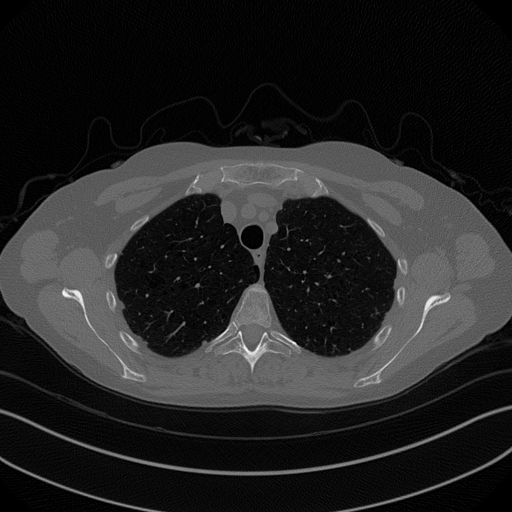
\includegraphics[width=0.3\textwidth]{media/2.png}
    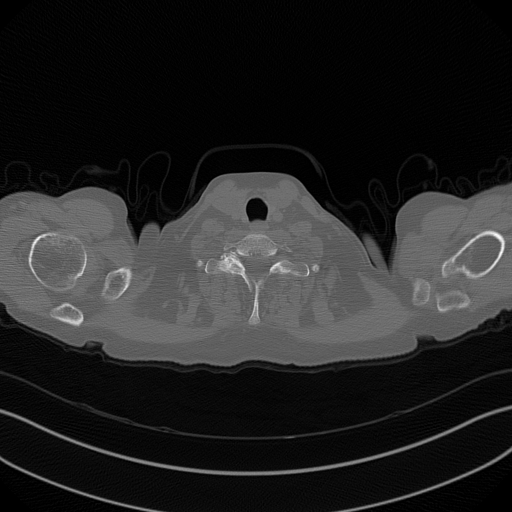
\includegraphics[width=0.3\textwidth]{media/3.png}
    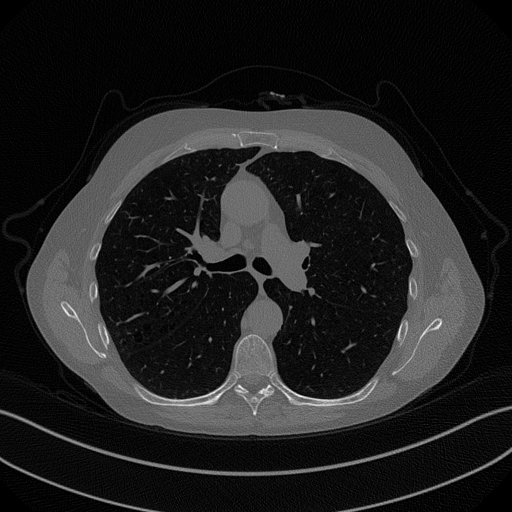
\includegraphics[width=0.3\textwidth]{media/100.png}
    \caption{Examples of CT slices from the Mayo Clinic dataset}
  \end{figure}  
  \end{itemize}
\end{frame}

% Frame 2: Conversion Pipeline
\begin{frame}[fragile]{Conversion Pipeline}
  Before applying augmentations, each image is converted using:
  \begin{enumerate}
    \item \textbf{Grayscale}: single channel via \texttt{transforms.Grayscale(num\_output\_channels=1)}
    \item \textbf{Resize}: to $128\times128$ pixels using bicubic interpolation
    \item \textbf{Normalization}: values scaled to $[-1,1]$ using mean $0.5$ and std $0.5$
  \end{enumerate}
  \vspace{0.5em}
  \begin{verbatim}
base_transform = transforms.Compose([
    transforms.Grayscale(1),
    transforms.Resize((128,128), interpolation=Image.BICUBIC),
    transforms.ToTensor(),
    transforms.Normalize([0.5], [0.5]),
])
  \end{verbatim}
\end{frame}

% Frame 3: Data Augmentation Types
\begin{frame}{Data Augmentation: Types}
  For each clean image, we apply the following transformations:
  \begin{itemize}
    \item \textbf{Fixed rotations}: $\pm5^\circ$ via \texttt{rotate\_fixed()}
    \item \textbf{Horizontal flip}: \texttt{horizontal\_flip()}
    \item \textbf{Gaussian noise}: mean $0$, std $10$ via \texttt{add\_gaussian\_noise()}
    \item \textbf{Salt-and-pepper noise}: probability $2\%$ via \texttt{add\_salt\_pepper()}
    \item \textbf{Brightness adjustment}: factor $1.2$ via \texttt{change\_brightness()}
    \item \textbf{Contrast adjustment}: factor $1.3$ via \texttt{change\_contrast()}
  \end{itemize}
\end{frame}
